% explain goal
% explain data set
% show problems data set


\slide{Image Segmentation}
{
% We want to introduce the problem:
%	- Tell about image segmentation
%		Segment image into several classes..?
%	What do we want to tell about image segmentation?
\begin{itemize}
	\item Old books, from 16th and 17th century (Dutch golden age)  are
scanned and digitally available
	\item For some, the text is available seperately
	\item Interesting idea: extract images to show those seperately as well
\end{itemize}
}

\subsection{Dataset}
% ik vind het best wel vreemd deze opdeling. Ik zou altijd 2 paginas laten
% zien, en nooit iets een probleem noemen
\slide{Dataset - Overview 1}
{
	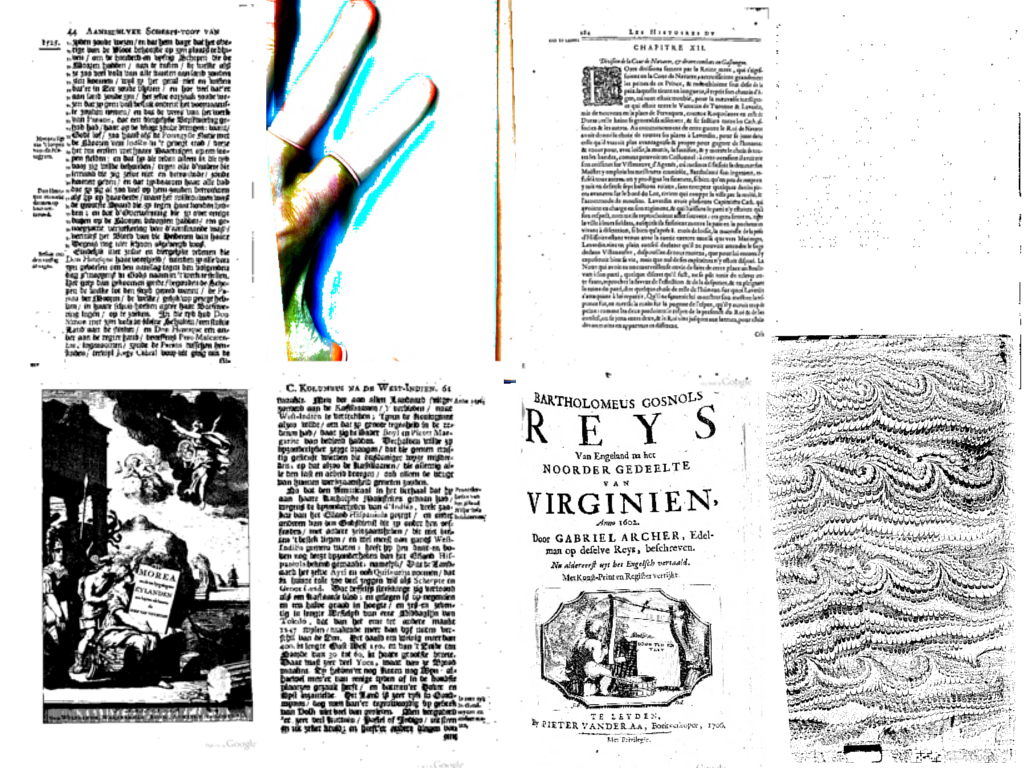
\includegraphics[width=.8\paperwidth]{resources/example1}
}
\slide{Dataset - Overview 2}
{
	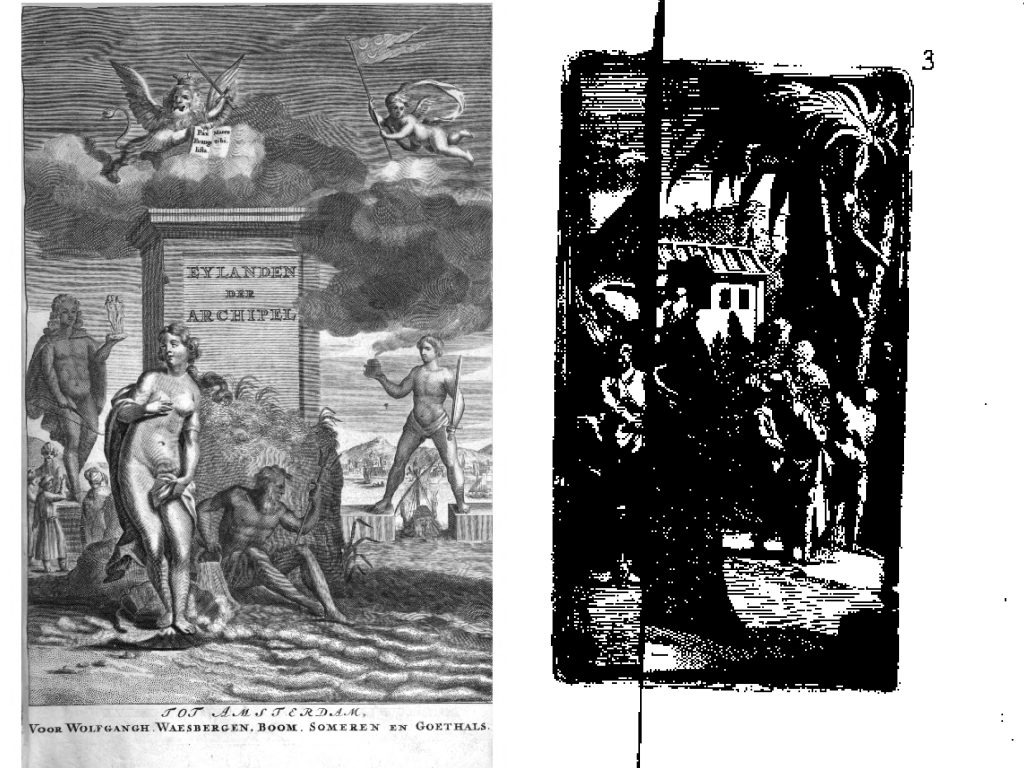
\includegraphics[width=.8\paperwidth]{resources/example2}
}


\begin{frame}[allowframebreaks]{HOG Examples}
	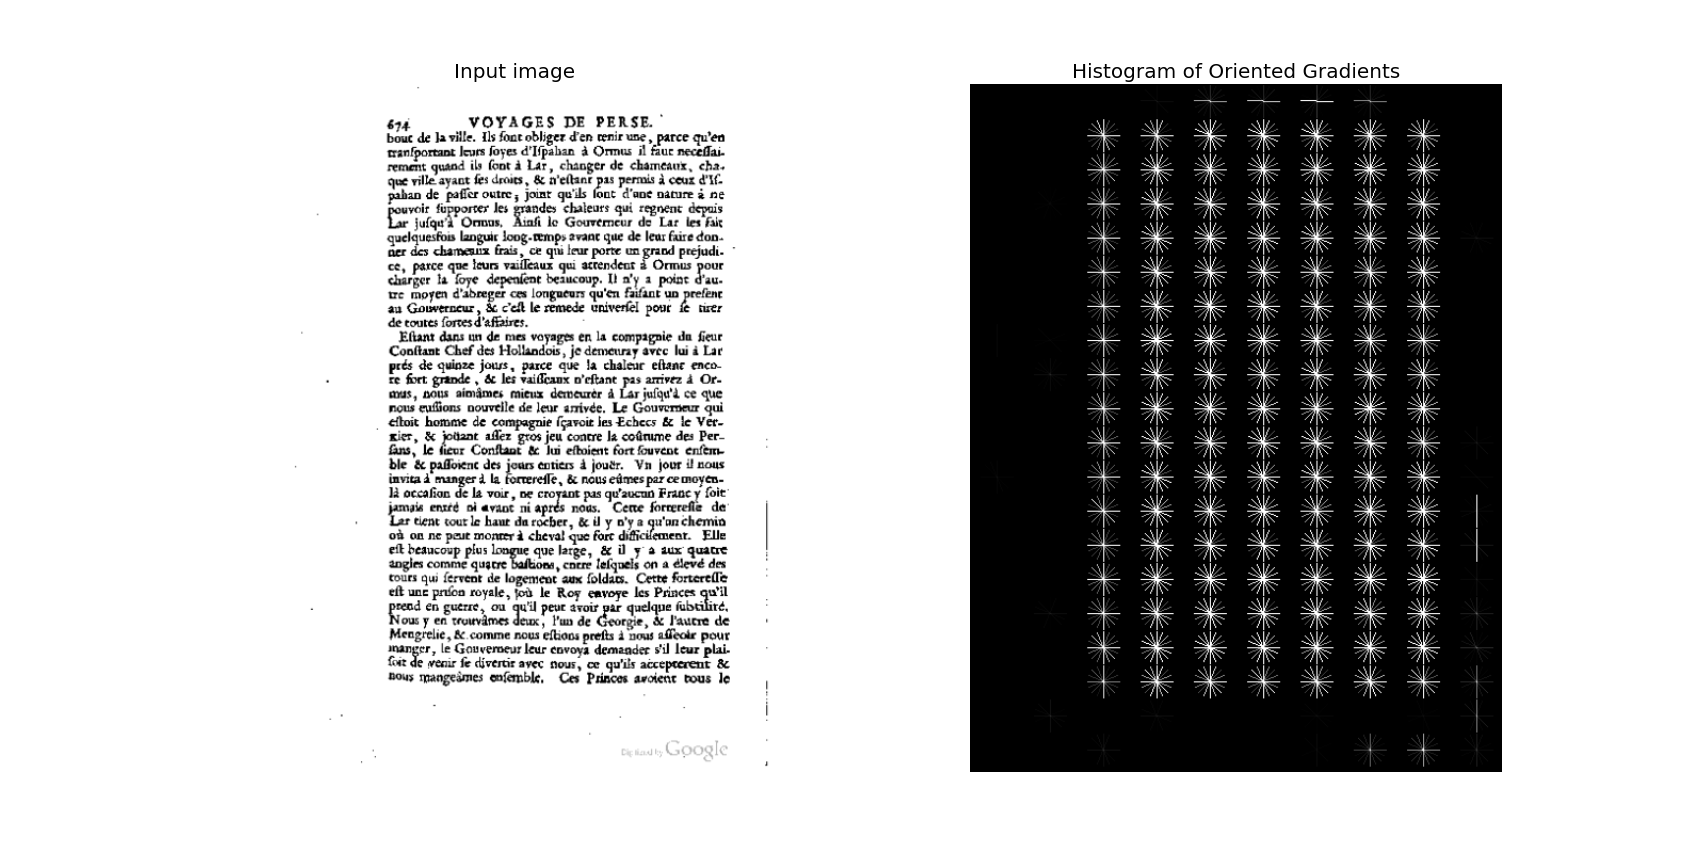
\includegraphics[trim=200px 0px 100px 0px, clip=true, width=.8\paperwidth]{resources/text1}\\
\framebreak
	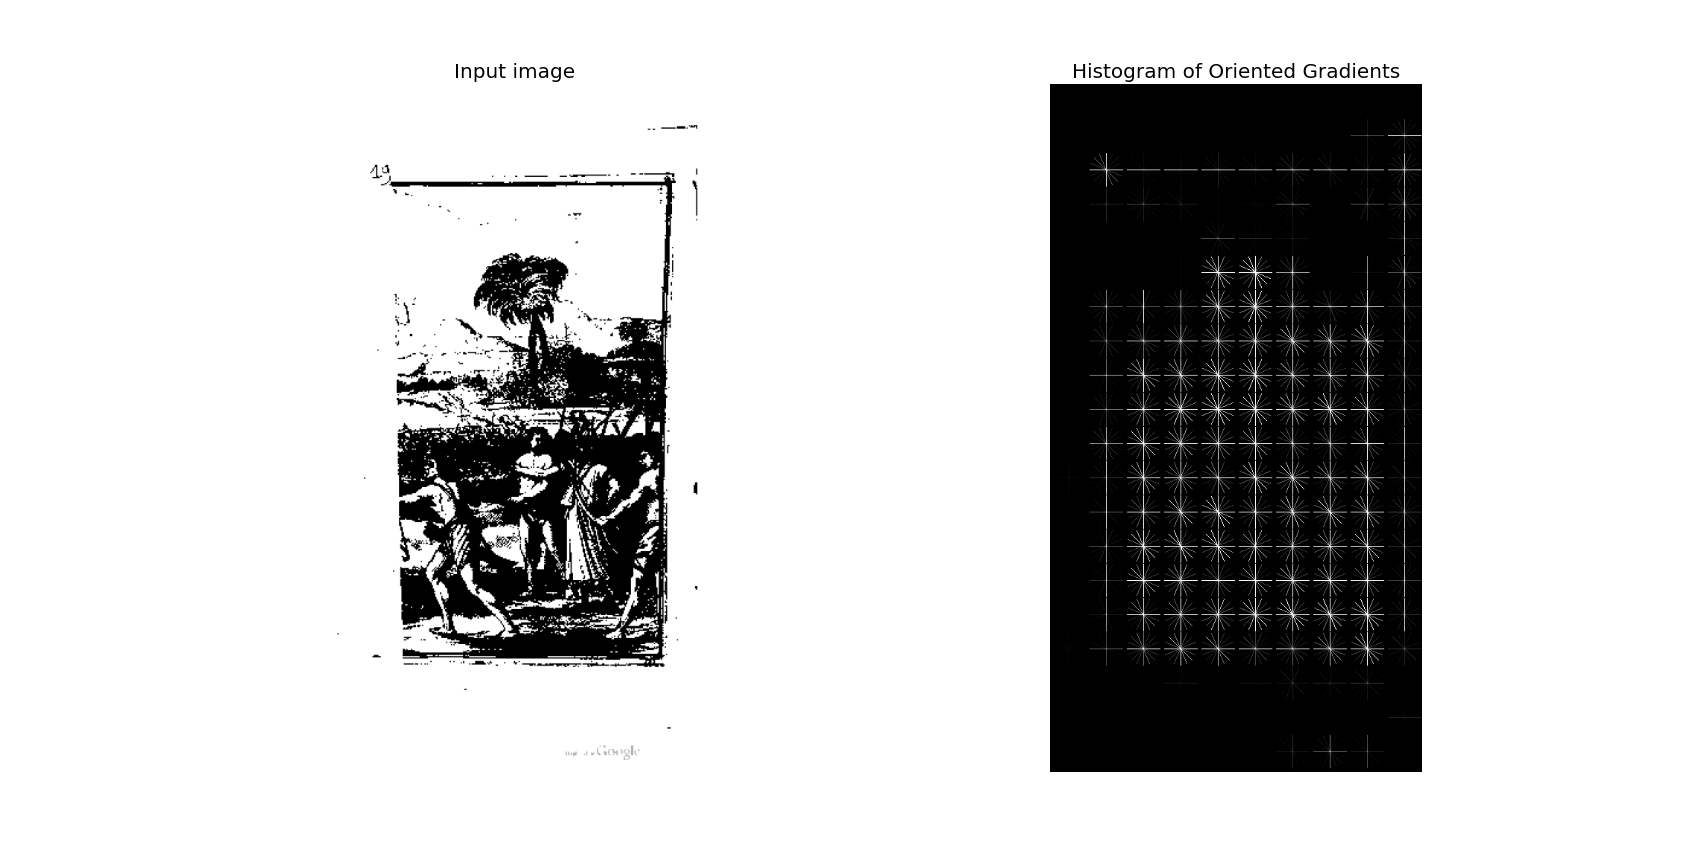
\includegraphics[trim=200px 0px 100px 0px, clip=true, width=.8\paperwidth]{resources/image1}\\
\framebreak
	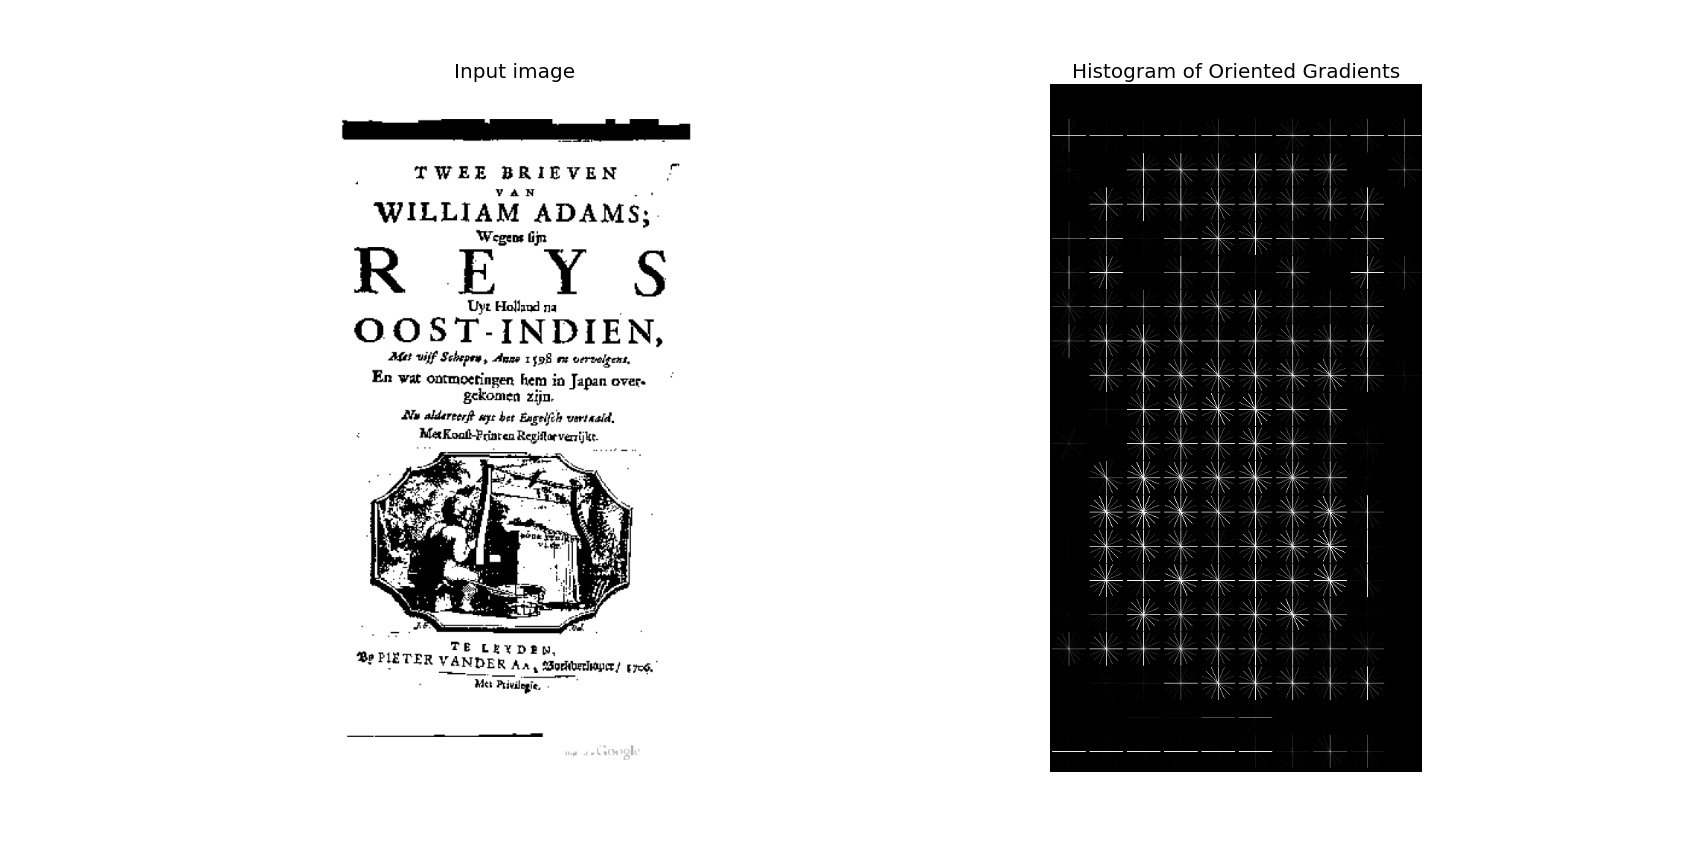
\includegraphics[trim=200px 0px 100px 0px, clip=true, width=.8\paperwidth]{resources/text_and_image1}
\end{frame}
